% Sequential versus simultaneous dynamic optimization. Authored 2026-09-14 for
% Lecture 7 Sec. XI, answering Alex's note after teaching:
%
%     "7-21. Before these two activities, it would be helpful to show a diagram
%      of simultaneous versus sequential. I am thinking a diagram that shows how
%      sequential iterates with a DAE/PDE integrator that also returns
%      derivatives."
%
% THE CONTRAST THE FIGURE HAS TO CARRY, because the two activities beneath it
% both turn on it:
%   * SEQUENTIAL keeps an integrator in the loop. The NLP only ever sees
%     (u, p); it never sees the states as variables. Every call hands back a
%     converged trajectory AND its sensitivities -- that is the part Alex asked
%     to draw, and it is why the method needs a differentiable integrator. So
%     every iterate is a feasible trajectory, and a legacy simulator that cannot
%     produce sensitivities cannot be used this way.
%   * SIMULTANEOUS has no integrator at all. The discretized states are decision
%     variables and the collocation equations are constraints, so the DAE is
%     satisfied only when the NLP converges -- there is no trajectory to look at
%     before then. That is the trade-off the Computational Note states in words.
%
% The three bullets of Sec. XI's second activity ("when would you NOT use
% simultaneous?") map onto the left panel: legacy simulator, hard-to-initialize
% DAE, and every-iterate-must-be-feasible.
%
% GREYSCALE. Okabe-Ito blue #0072B2 for the optimizer and orange #E69F00 for
% the integrator, but nothing is carried by colour: the two boxes differ in
% SHAPE (rounded vs sharp), the loop is drawn with arrows on both legs, and each
% panel carries a text verdict underneath. Prints legibly in pure black.
%
% TIKZ LIBRARIES. arrows.meta and positioning, both already loaded by the pack's
% preamble for the other Lecture 7 figures.

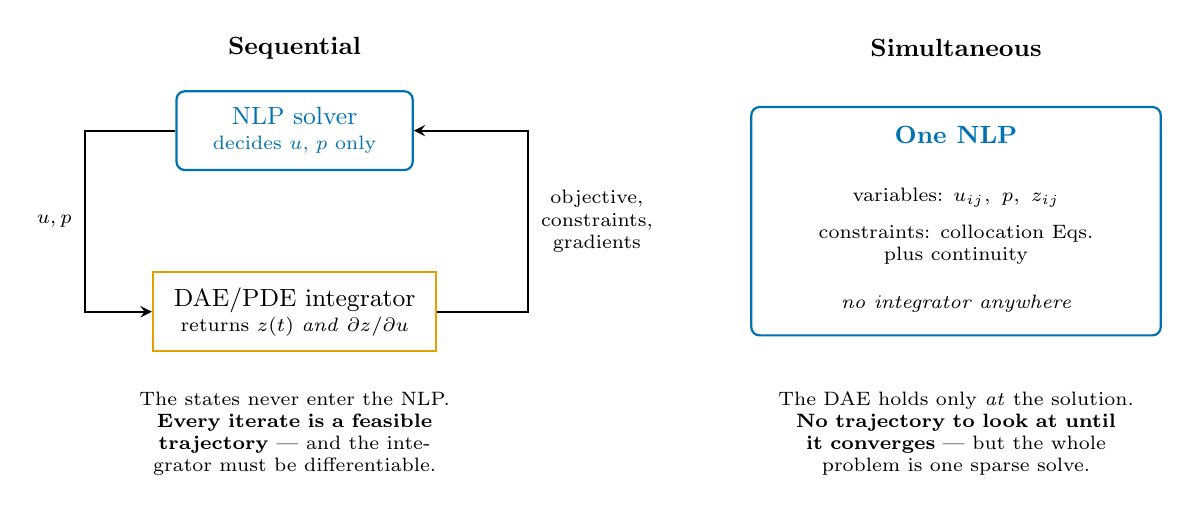
\begin{tikzpicture}[
  font=\small,
  box/.style={draw, thick, rounded corners=3pt, align=center,
              minimum height=1.0cm, inner xsep=6pt},
  sharp/.style={draw, thick, align=center, minimum height=1.0cm, inner xsep=6pt},
  lbl/.style={font=\scriptsize, align=center},
  >=stealth
]
  \definecolor{svblue}{HTML}{0072B2}
  \definecolor{svorange}{HTML}{E69F00}

  % ================= LEFT PANEL: SEQUENTIAL =================
  \node[lbl, font=\small\bfseries] at (0,2.65) {Sequential};

  \node[box, draw=svblue, text=svblue, minimum width=3.0cm] (nlp1) at (0,1.6)
    {NLP solver\\[-2pt]{\scriptsize decides $u$, $p$ only}};
  \node[sharp, draw=svorange, minimum width=3.6cm] (int) at (0,-0.7)
    {DAE/PDE integrator\\[-2pt]{\scriptsize returns $z(t)$ \emph{and}
     $\partial z/\partial u$}};

  \draw[->, thick] (nlp1.west) -- ++(-1.15,0) |- (int.west)
    node[lbl, pos=0.25, left=1pt] {$u,p$};
  \draw[->, thick] (int.east) -- ++(1.15,0) |- (nlp1.east)
    node[lbl, pos=0.25, right=1pt] {objective,\\constraints,\\gradients};

  \node[lbl, text width=5.0cm] at (0,-2.25)
    {The states never enter the NLP.\\
     \textbf{Every iterate is a feasible trajectory} --- and the integrator
     must be differentiable.};

  % ================= RIGHT PANEL: SIMULTANEOUS =================
  \node[lbl, font=\small\bfseries] at (8.4,2.65) {Simultaneous};

  \node[box, draw=svblue, text=svblue, minimum width=5.2cm, minimum height=2.9cm]
    (nlp2) at (8.4,0.45) {};
  \node[lbl, text=svblue, font=\small\bfseries] at (8.4,1.55) {One NLP};
  \node[lbl] at (8.4,0.75) {variables: $u_{ij},\ p,\ z_{ij}$};
  \node[lbl] at (8.4,0.15)
    {constraints: collocation Eqs.~\\ plus continuity};
  \node[lbl, font=\scriptsize\itshape] at (8.4,-0.6) {no integrator anywhere};

  \node[lbl, text width=5.0cm] at (8.4,-2.25)
    {The DAE holds only \emph{at} the solution.\\
     \textbf{No trajectory to look at until it converges} --- but the whole
     problem is one sparse solve.};
\end{tikzpicture}
